\section{【实现】设计进程控制块}\label{ux5b9eux73b0ux8bbeux8ba1ux8fdbux7a0bux63a7ux5236ux5757}

在proj10中,进程管理信息用struct
proc\_struct表示,在kern/process/proc.h中定义如下:

\begin{lstlisting}
struct proc_struct {
    enum proc_state state;        // Process state
    int pid;                        // Process ID
    int runs;                       // the running times of Proces
    uintptr_t kstack;             // Process kernel stack
    volatile bool need_resched; // need to be rescheduled to release CPU?
    struct proc_struct *parent; // the parent process
    struct mm_struct *mm;        // Process's memory management field
    struct context context;     // Switch here to run process
    struct trapframe *tf;       // Trap frame for current interrupt
    uintptr_t cr3;               // the base addr of Page Directroy Table(PDT)
    uint32_t flags;              // Process flag
    char name[PROC_NAME_LEN + 1];  // Process name
    list_entry_t list_link;    // Process link list 
    list_entry_t hash_link;    // Process hash list
};
\end{lstlisting}

在上述域中,与进程管理各个相关层面的对应关系如下表所示:

\begin{figure}[htbp]
\centering
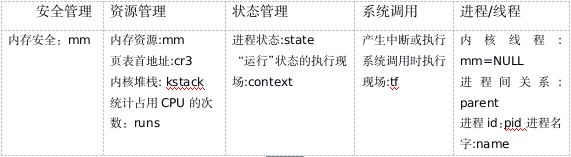
\includegraphics{figures/0_2.png}
\caption{0\_2}
\end{figure}

下面重点解释一下几个比较重要的域:

\begin{itemize}
\tightlist
\item
  mm
  :内存管理的信息,包括内存映射列表、页表指针等。mm里有个很重要的项pgdir,记录的是该进程使用的一级页表的物理地址。
\item
  state:进程所处的状态。
\item
  parent
  :用户进程的父进程(创建它的进程)。在所有进程中,只有一个进程没有父进程,就是内核创建的第一个内核线程idleproc。内核根据这个父子关系建立进程的树形结构,用于维护一些特殊的操作,例如确定哪些进程是否可以对另外一些进程进行什么样的操作等等。
\item
  context:进程的上下文,用于进程切换(参见switch.S)。在 ucore
  中,所有的进程在内核中也是相对独立的(例如独立的内核堆栈以及上下文等等)。使用
  context
  保存寄存器的目的就在于在内核态中能够进行上下文之间的切换。实际利用context进行上下文切换的函数是switch\_to,在kern/process/switch.S中定义。
\item
  tf:中断帧的指针,总是指向内核栈的某个位置:当进程从用户空间跳到内核空间时,中断帧记录了进程在被中断前的状态。当内核需要跳回用户空间时,需要调整中断帧以恢复让进程继续执行的各寄存器值。除此之外,ucore
  内核允许嵌套中断。因此为了保证嵌套中断发生时tf 总是能够指向当前的
  trapframe,ucore 在内核桟上维护了 tf 的链,可以参考 trap.c::trap函数
  做进一步的了解。
\item
  cr3: cr3 保存页表的物理地址,目的就是进程切换的时候方便直接使用 lcr3
  实现页表切换,避免每次都根据 mm 来计算 cr3。mm
  数据结构是用来实现用户空间的虚存管理的,但是内核线程没有用户空间,它执行的只是内核中的一小段代码(通常是一小段函数),所以它没有
  mm 结构,也就是NULL。当某个进程是一个普通用户态进程的时候,PCB 中的
  cr3 就是 mm 中页表(pgdir)的物理地址;而当它是内核线程的时候,cr3
  等于 boot\_cr3。
  而boot\_cr3指向了ucore启动时建立好的饿内核虚拟空间的页目录表首地址。
\item
  kstack:
  每个进程都有一个内核桟,并且位于内核地址空间的不同位置。对于内核线程,该桟就是运行时的程序使用的桟;而对于普通进程,该桟是发生特权级改变的时候使保存被打断的硬件信息用的桟。Ucore在创建进程时分配了
  2 个连续的物理页(参见
  memlayout.h)作为内核栈的空间。这个桟很小,所以内核中的代码应该尽可能的紧凑,并且避免在桟上分配大的数据结构,以免桟溢出,导致系统崩溃。kstack记录了分配给该进程/线程的内核桟的位置。主要作用有以下几点。首先,当内核准备从一个进程切换到另一个的时候,需要根据
  kstack 的值正确的设置好 tss (可以回顾一下在lab1中讲述的 tss
  在中断处理过程中的作用),以便在进程切换以后再发生中断时能够使用正确的桟。其次,内核桟位于内核地址空间,并且是不共享的(每个进程/线程都拥有自己的内核桟),因此不受到
  mm 的管理,当进程退出的时候,内核能够根据 kstack
  的值快速定位桟的位置并进行回收。ucore 的这种内核桟的设计借鉴的是 linux
  的方法(但由于内存管理实现的差异,它实现的远不如 linux
  的灵活),它使得每个进程/线程的内核桟在不同的位置,这样从某种程度上方便调试,但同时也使得内核对栈溢出变得十分不敏感,因为一旦发生溢出,它极可能污染内核中其它的数据使得内核崩溃。如果能够通过页表,将所有进程的内核桟映射到固定的地址上去,能够避免这种问题,但又会使得进程切换过程中对桟的修改变得相当繁琐。感兴趣的同学可以参考
  linux kernel 的代码对此进行尝试。
\end{itemize}

为了管理系统中所有的进程控制块,ucore维护了如下全局变量(位于kern/process/proc.c):

\begin{itemize}
\tightlist
\item
  static struct proc *current;
  //当前占用CPU,处于``运行''状态进程控制块指针。通常这个变量是只读的,只有在进程切换的时候才进行修改,并且整个切换和修改过程需要保证操作的原子性,目前至少需要屏蔽中断,可以参考
  switch\_to 的实现,后面也会介绍到。linux
  的实现很有意思,它将进程控制块放在进程内核桟的底部,这使得任何时候
  current
  都可以根据内核桟的位置计算出来的,而不用维护一个全局变量。这样使得一致性的维护以及多核的实现变得十分的简单和高效。感兴趣的同学可以参考
  linux kernel 的代码。
\item
  static struct proc *initproc; //指向第一个用户态进程(proj10以后)
\item
  static list\_entry\_t hash\_list{[}HASH\_LIST\_SIZE{]};
  //所有进程控制块的哈希表,这样proc\_struct中的域hash\_link将基于pid链接入这个哈希表中。
\item
  list\_entry\_t proc\_list;//
  所有进程控制块的双向线性列表,这样proc\_struct中的域list\_link将链接入这个链表中。
\end{itemize}
